%% jan. 4, 2011  items to fix:
%% notation for math and reference to images.
%% how include eps figures.
%% make all the little figures (search for eps) in a common, nice matlab way for the
%% example filtering operations.

\chapter{Blur Filters}
\label{chap:blur_filters}




\section{Introduction}

Blur filters are low-pass filters. They remove the high spatial-frequency content from an image leaving only the low-frequency spatial components. The result is an image that has lost details and that looks {\bf blurry}. Image blur has many applications in computer graphics and computer vision. It can be used to reduce noise (as shown in \fig{\ref{fig:stop_256_noise_3}}), to reveal image structures at different scales, or for upsampling and downsampling images.


\begin{figure}[h]
\centerline{
\includegraphics[width=.475\linewidth]{figures/blur_filters/stop_256_noise_3.jpg}~
\includegraphics[width=.475\linewidth]{figures/blur_filters/stop_256_blur_3.jpg}
}
\caption{Image denoising by blurring (each color channel is filtered independently). The noise is mostly gone, but also many image details are gone. Image blurring removes all the high-frequency content in the image.}
\label{fig:stop_256_noise_3}
\end{figure}

Blurring is implemented by computing local averages over small neighborhoods of input pixel values. This can be done by a convolution. However, there are nonlinear approaches for removing image details such as anisotropic diffusion \cite{Perona1990} and bilateral filtering \cite{Paris2009}. These nonlinear blurring techniques can be useful when we want to remove noise while preserving some image details such as contours.

In this chapter we will focus on linear filters for image blurring. We will describe three popular families of blurring filters, discussing properties and limitations. 

%Figure: Picture behind bars, show that blurring removes the bars?

%Figure: Can we reveal some global structure in an image not clearly visible?

%
%
%Michelson contrast:
%\begin{equation}
%(Imax-Imin)/(Imax+Imin)  
%\end{equation}
%
%Weber contrast:  $\Delta I / I$.
%


%We will start by studying several important linear spatially invariant filters. These filters can be implemented as convolutions between an input image and a linear kernel.

\section{Box Filter}


Let's start with a very simple low-pass filter, the box filter.  
\index{Filter!Box filter} In \sect{\ref{sec:box_function}} we presented the box function. The box filter uses a box function as the convolution kernel. 
The box convolution kernel can be written as:
%\begin{equation}
%h_{N,M} \left[n,m \right] = 
%\begin{cases}
%    1       & \quad \text{if } -N \leq n \leq N  \text{~and~}  -M \leq m \leq M\\
%    0       & \quad \text{otherwise.} 
%  \end{cases}
%\end{equation}

\begin{equation}
\text{box}_{N,M} \left[n,m \right] = 
\begin{cases}
    1       & \quad \text{if } -N \leq n \leq N  \text{~and~}  -M \leq m \leq M\\
    0       & \quad \text{otherwise.} 
  \end{cases}
\end{equation}

\marginnote{The box filter with $N=M=1$ is:
\begin{center}
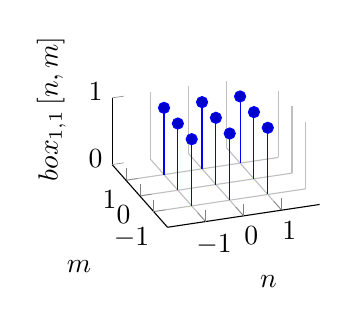
\begin{tikzpicture} 
\begin{axis}[width=120pt,height=100pt,
	mesh/ordering=y varies,
 	%axis x line=middle, 
	%axis y line=middle, 
	%axis z line=middle, 
	%tick align=center,
    xmajorgrids=true,
    ymajorgrids=true,
    zmajorgrids=false,
    zminorgrids=false,
    axis lines*=left, 
    %grid=both%,restrict z to domain*=0:1
	view={-20}{45},
	xmin=-2, xmax=2,
	xtick={-1, 0, 1},
	ymin=-2, ymax=2,
	ytick={ -1, 0, 1}, 
	zmin=0, zmax=1,
	ztick={0, 1}, 
    xlabel={$n$}, 
    ylabel={$m$}, 
    zlabel={$\text{box}_{1,1} \left[n, m \right]$}
	]  
\addplot3+[ycomb]
coordinates { 
%(-2,-2,0) (-2,-1,0) (-2,0,0) (-2,1,0) (-2,2,0)
%(-1,-2,0)  (-1,2,0)
%(0,-2,0)  (0,2,0)
%(1,-2,0)  (1,2,0)
%(2,-2,0) (2,-1,0) (2,0,0) (2,1,0) (2,2,0)
(-1,-1,1) (-1,0,1) (-1,1,1)  (0,-1,1) (0,0,1) (0,1,1)  (1,-1,1) (1,0,1) (1,1,1)
};
\end{axis} 
\end{tikzpicture}
\end{center}
%\caption{A discrete 2D signal.} 
%\label{fig:disc2Dsignal_plot}
%\end{figure}
}

Filtering an input image, $\imgin$, with a box filter results in the following:
\begin{eqnarray}
\imgout \left[n,m\right] &=& \text{box}_{N,M} \left[n,m\right] \circ \imgin \left[n,m\right] \nonumber \\
&=&  \sum_{k,l} \imgin \left[n-k,m-l \right] \text{box}_{N,M} \left[k,l \right] \nonumber \\
&=&  \sum_{k=-N}^N \sum_{l=-M}^M \imgin \left[n-k,m-l \right]
\end{eqnarray}
That is, the output value on each location $(n,m)$ is the sum of the input pixels within the rectangle around that location.  


Visually, filtering an image with the box filter results in blurring the picture. \Fig{\ref{fig:convExamps2}} shows some box filters and the corresponding output images (after normalizing the box filter coefficients so that they sum to 1). \Fig{\ref{fig:convExamps2}}{a} shows an image convolved with a squared box kernel (i.e., $N=M$). 

Figures \ref{fig:convExamps2}(b) and \ref{fig:convExamps2}(c)  show the results of blurring in just one direction. Blur happens very often in real life. It happens when we look at something very far away, or at some detail inside a picture, or when we remove our eyeglasses (or wear some that are not ours). 


\begin{figure}[t]
$
\begin{array}{cccc}
\includegraphics[width=.18\linewidth]{figures/spatial_filters/img1.jpg}
&
%\text{a)}
\includegraphics[width=.05\linewidth]{figures/spatial_filters/street_square_kernel.jpg}
%&
~
\includegraphics[width=.18\linewidth]{figures/spatial_filters/street_square.jpg}
&
%\text{b)}
\includegraphics[width=.05\linewidth]{figures/spatial_filters/street_horizontal_kernel.jpg}
%&
~
\includegraphics[width=.18\linewidth]{figures/spatial_filters/street_horizontal.jpg}
&
%\text{c)}
\includegraphics[width=.05\linewidth]{figures/spatial_filters/street_vertical_kernel.jpg}
%&
~
\includegraphics[width=.18\linewidth]{figures/spatial_filters/street_vertical.jpg}
\\
\text{(a)}&\text{(b)}&\text{(c)}&\text{(d)}
\end{array}
$
\caption{(a) Input image. (b) Blurring with a square, (c) a horizontal, and
  (d) a vertical line. Each color channel is filtered independently.
} 
\label{fig:convExamps2}
\end{figure}

\subsection{Properties}

The box filter is a low-pass filter. That is, it attenuates the high spatial-frequency content of the input image. 

As we already mentioned in \sect{\ref{sec:box_function}}, the two-dimensional (2D) box filter is separable as it can be written as the convolution of two 1D kernels: $\text{box}_{N,M} \left[n,m \right]  = \text{box}_{N,0} \circ \text{box}_{0,M}$. When the box is large, it can be implemented efficiently using the integral image \cite{Viola01}.


One important property of a low-pass filter is the {\bf DC gain}\index{DC gain}\footnote{Remember that the DC value of a signal is its mean value. DC is an old name derived from Direct Current.}, that is, the gain it has for a constant value input (i.e., the lowest possible input frequency). If the input signal is a constant, i.e., $\img[n,m] = a$, where $a$ is a real number, the result of convolving the image with the box filter $h_{N,M}$ is also a constant:
\begin{equation}
\imgout \left[n,m\right] = \sum_{k,l} a \text{box}_{N,M} \left[k,l \right] = a \sum_{k,l} \text{box}_{N,M} \left[k,l \right]  = a (2N+1)(2M+1)
\end{equation}

In general, The DC gain of an arbitrary filter $h [n,m]$ is the sum of  its kernel values, 
\begin{equation}
\text{DC~gain} = \sum_{n,m} h [n,m]
\end{equation}
In the example of the box filter with $N=1$, the DC gain is 3. 

In the frequency domain, the DC gain of a filter refers to its gain at frequency of 0. This gain is represented by the value $H[0,0]$, where $H$ is the result of applying the Discrete Fourier Transform (DFT) to the filter's kernel $h$. This can be easily proven by checking the definition of the DFT and setting the spatial frequencies to zero. One can verify in \fig{\ref{fig:boxfilter}} that the value of $\left| \text{Box}_1[0] \right|$ is $3$. The DC gain of a filter will change the mean value of the input signal. 

%of a filter is the gain of the filter for the frequency 0. That is, the DC gain is also the value of $H[0,0]$, where $H$ is the Discrete Fourier transform of the filter kernel $h$. This can be easily proven by checking the definition of the DFT and setting the spatial frequencies to zero. One can verify in \fig{\ref{fig:boxfilter}} that the value of $\left| \text{Box}_1[0] \right|$ is $3$. 



\begin{figure}[t]
\centerline{
%\begin{center}
%\[
%\begin{array}{cc}
%\text{(a)}
\sublabel{a}{
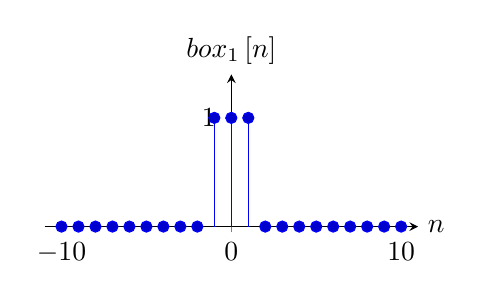
\begin{tikzpicture}
\begin{axis} [width=180pt,height=100pt,
	axis x line=bottom, 
	axis y line=middle, 
	tick align=center,
	every axis x label/.style={at={(current axis.right of origin)},anchor=west},
	every axis y label/.style={at={(current axis.above origin)}, anchor=north east,above=0mm},
	xmin=-11, xmax=11,
	xtick={-10, 0, 10},
	xlabel=$n$,
	ymin=0, ymax=1.4,
	ytick={0,...,1},
	ylabel={$\text{box}_1 \left[n\right]$}]
\addplot+[ycomb] plot coordinates {(-10,0) (-9,0) (-8,0) (-7,0) (-6,0) (-5,0) (-4,0) (-3,0) (-2,0) (-1,1) (0,1) (1,1) (2,0) (3,0) (4,0) (5,0) (6,0) (7,0) (8,0) (9,0) (10,0)};
\end{axis} 
\end{tikzpicture}
}
\sublabel{b}{
%\text{(b)}
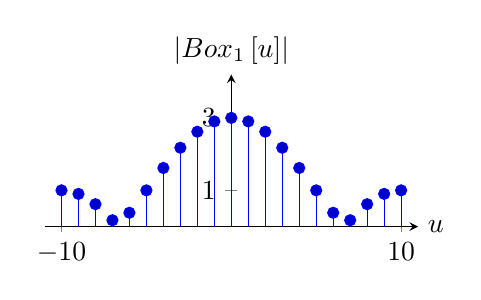
\begin{tikzpicture}
\begin{axis} [width=180pt,height=100pt,
	axis x line=middle, 
	axis y line=middle, 
	tick align=center,
	every axis x label/.style={at={(current axis.right of origin)},anchor=west},
	every axis y label/.style={at={(current axis.above origin)}, anchor=north east,above=0mm},
	xmin=-11, xmax=11,
	xtick={-10, 0,10},
	xlabel=$u$,
	ymin=0, ymax=4.2,
	ytick={0,1,3},
	ylabel={$\left| \text{Box}_1 \left[ u \right] \right|$},
	color=black]
 \addplot+[ycomb,domain=-10:10,samples=21,samples y=0] 
 ({x}, {abs(1+2*cos(deg(2*pi*x*1/20)))}); 
\end{axis}
\end{tikzpicture}
%\end{array}
%\]
%\end{center}
}
}
\caption{(a) A one-dimensional (1D) box filter ($\left[1,1,1\right]$), and (b) its Fourier transform over 20 samples. Note that the frequency gain is not monotonically decreasing with spatial frequency.} 
\label{fig:boxfilter}
\end{figure}

When designing blur kernels (low-pass filters), we generally want to have a DC gain of 1. The reason is that if we have an image with grayscale levels in the range of 0 to 256 and with an average around 128, we will want to preserve the same mean value in the output. For this reason, in most applications, we will normalize the kernel values so that they sum 1. In the case of the box filter this means dividing the kernel values by $(2N+1)(2M+1)$. 


\subsection{Limitations}

The box filter is simple to implement and to understand, but it has a number of limitations:

\begin{itemize}
\item {The box filter is not a perfect blurring filter. A blur filter should attenuate high spatial frequencies with stronger attenuation for higher spatial frequencies. However, if you consider the highest spatial frequency, which will be an oscillating signal that takes successively on the values 1 and $-1$: $\left[..., 1, -1, 1, -1, 1, -1, ... \right]$ when filtered with the box filter $\text{box}_{1}$ the result is the same oscillating signal! However, if you filter a wave with lower frequency such as $\left[..., 0.5, 0.5, -1, 0.5, 0.5, -1, ... \right]$ then the result is $\left[..., 0,0,0,0, ...\right]$. Therefore, the attenuation is not monotonic with spatial frequency as it is shown in \fig{\ref{fig:boxfilter}}. This is not a desirable behavior for a blurring filter and it can cause artifacts to appear. This could be addressed using an even size box filter $\left[1,1 \right]$. However, an even box filter is not centered around the origin and the output image will have a half-pixel translation. Therefore, odd filter sizes are preferred.}

\marginnote{The oscillating signal\\[6pt]
\centerline{
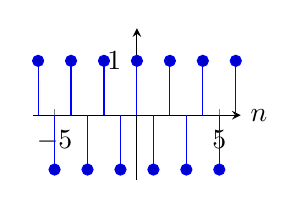
\begin{tikzpicture}
\begin{axis} [width=120pt,height=100pt,
	axis x line=middle, 
	axis y line=middle, 
	tick align=center,
	every axis x label/.style={at={(current axis.right of origin)},anchor=west},
	every axis y label/.style={at={(current axis.above origin)}, anchor=north east,above=0mm},
	xmin=-6.3, xmax=6.3,
	%xtick={-6, -2,2,4, 6},
	xlabel=$n$,
	ymin=-1.2, ymax=1.6,
	ytick={1},
	%ylabel={$\text{box}_1 \left[n\right]$}
 ]
\addplot+[ycomb] plot coordinates {(-6,1) (-5,-1) (-4,1) (-3,-1) (-2,1) (-1,-1) (0,1) (1,-1) (2,1) (3,-1) (4,1) (5,-1) (6,1)};
\end{axis} 
\end{tikzpicture}
}
\\[6pt]
convolved with the kernel $[1,1,1]$ results in:
\\[6pt]
\centerline{
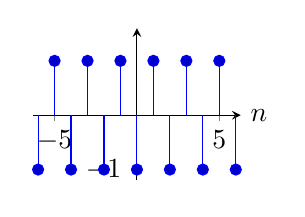
\begin{tikzpicture}
\begin{axis} [width=120pt,height=100pt,
	axis x line=middle, 
	axis y line=middle, 
	tick align=center,
	every axis x label/.style={at={(current axis.right of origin)},anchor=west},
	every axis y label/.style={at={(current axis.above origin)}, anchor=north east,above=0mm},
	xmin=-6.3, xmax=6.3,
	%xtick={-6, -2,2,4, 6},
	xlabel=$n$,
	ymin=-1.2, ymax=1.6,
	ytick={-1},
	%ylabel={$\text{box}_1 \left[n\right]$}
 ]
\addplot+[ycomb] plot coordinates {(-6,-1) (-5,1) (-4,-1) (-3,1) (-2,-1) (-1,1) (0,-1) (1,1) (2,-1) (3,1) (4,-1) (5,1) (6,-1)};
\end{axis} 
\end{tikzpicture}
}
}[-.3in]
\item {If you convolve two boxes you do not get another box. Instead you get a triangle. You can easily check this by convolving two box filters. For instance, in the simple case where $N=1, M=0$:
\begin{equation}
\text{box}_{1,0} \circ \text{box}_{1,0} = \left[1, 1, 1\right] \circ \left[1, 1, 1\right] = \left[1,2,3,2,1\right]
\end{equation}
the output  is a {\bf triangular filter} 
\index{Filter!Triangular filter}
with length $2\times L-1$, with $L=3$ the length of the box filter. When convolving two box filters of different length the result will be a truncated triangle.
Although that is not a problem at first sight, it means that if you blur an image twice with box filters, what you get is not the equivalent to blurring only once with a larger box filter.}
\end{itemize}



The next low-pass filter addresses both of these issues.

\section{Gaussian Filter}
\label{sec:spt_gaussian}

One of the important blurring (low-pass) filters in computer vision is the Gaussian filter. 
The Gaussian filter is important because it is a good model for many naturally occurring filters. It also has a number of properties, as we will discuss here, that make it unique. 

The Gaussian distribution is defined in continuous variables. In one dimension:
\index{Filter!Gaussian filter}
\begin{equation}
g(x; \sigma) = \frac{1}{\sqrt{2 \pi \sigma^2}} \exp{ \left( -\frac{x^2}{2 \sigma^2} \right) }
\label{eq:gauss1dcont}
\end{equation}
and in two dimensions:
\begin{equation}
g(x,y; \sigma) = \frac{1}{2 \pi \sigma^2} \exp{ \left(-\frac{x^2 +
   y^2}{2 \sigma^2} \right) }
\label{eq:gauss2dcont}
\end{equation}
The parameter $\sigma$ adjusts the spatial extend of the Gaussian. The normalization constant is set so that the function integrates to 1. The Gaussian kernel is positive and symmetric (a zero-phase filter).




\subsection{Discretization}



In order to use this filter in practice we need to consider discrete locations and also approximate the function by a finite support function. In practice, we only need to consider samples within three standard deviations $x \in (-3\sigma, 3\sigma)$. At $3\sigma$ the amplitude of the Gaussian filter is around 1 percent of its central value. Unfortunately, many of the properties of the Gaussian filter that we will discuss later are only true in the continuous domain and are only approximated when using its discrete form. 

For a given standard deviation parameter, $\sigma$, the discretized Gaussian kernel is $g \left[n, m; \sigma \right]$:
\index{Filter!Gaussian filter!Discrete}
\begin{equation}
g \left[ n,m; \sigma \right] = \exp{ \left( -\frac{n^2 + m^2}{2 \sigma^2} \right) }
\label{eq:gauss2d}
\end{equation}
We have removed the normalization constant as the sum of the discrete Gaussian will be different from the integral of the continuous function. So here we prefer to define the form in which the value at the origin is 1. In practice, we should normalize the discrete Gaussian by the sum of its values to make sure that the DC gain is 1. 

\marginnote{1D Gaussian with $\sigma=1$ and its discretized version:
\\[6pt]
\centerline{
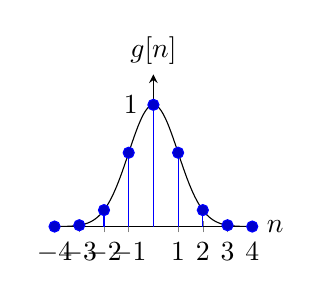
\begin{tikzpicture}
\begin{axis} [width=120pt,height=100pt,
	axis x line=middle, 
	axis y line=middle, 
	tick align=center,
	every axis x label/.style={at={(current axis.right of origin)},anchor=west},
	every axis y label/.style={at={(current axis.above origin)}, anchor=north east,above=0mm},
	xmin=-4.2, xmax=4.2,
	xtick={-4, -3, -2, -1, 0, 1, 2, 3, 4},
	xlabel=$n$,
	ymin=0, ymax=1.25,
	ytick={0,1},
	ylabel={$g[n]$}]
\addplot+[ycomb,domain=-4:4,samples=9,samples y=0] 
 ({x}, {exp(-x*x/(2*(1)^2)}); 
\addplot[domain=-4:4,samples=101,samples y=0] 
 ({x}, {exp(-x*x/(2*(1)^2)}); 
\end{axis} 
\end{tikzpicture}
}
}[0in]

By adjusting the standard deviation, $\sigma$, of the Gaussian, it is possible to adjust the level of image detail
that appears in the blurred image. \Fig{\ref{fig:zebragaussian}} shows the result of narrow and wider Gaussians applied to an image. 
 

\begin{figure}[t]
%$
%\begin{array}{ccc}
%\text{(a)}
\centerline{
\sublabel{a}{
\includegraphics[width=.28\linewidth]{figures/spatial_filters/gausian_zebra_c_2.jpg}}
\sublabel{b}{
\includegraphics[width=.28\linewidth]{figures/spatial_filters/gausian_zebra_c_4.jpg}}
\sublabel{c}{
\includegraphics[width=.28\linewidth]{figures/spatial_filters/gausian_zebra_c_8.jpg}}
}
\centerline{
%\\
\sublabel{d}{
\includegraphics[width=.28\linewidth]{figures/spatial_filters/gausian_c_2plot.jpg}}
\sublabel{e}{
\includegraphics[width=.28\linewidth]{figures/spatial_filters/gausian_c_4plot.jpg}}
\sublabel{f}{
\includegraphics[width=.28\linewidth]{figures/spatial_filters/gausian_c_8plot.jpg}}
%\end{array}
%$
}
\caption{An image filtered with three Gaussians with standard deviations: (a) $\sigma=2$, (b) $\sigma=4$, and (c) $\sigma=8$. Plots (d--f) show the three Gaussians over the same spatial support as the image. The discrete Gaussians are approximated by sampling the continuous Gaussian. The convolutions are performed with mirror boundary conditions.} 
\label{fig:zebragaussian}
\end{figure}


The $n$-dimensional Gaussian filter has the additional computational advantage that it can
be applied as a concatenation of $n$ 1D Gaussian filters.  This can be
seen by writing the 2D Gaussian, \eqn{\ref{eq:gauss2d}}, in the
convolution equation, \eqn{\ref{eq:2dconv}}.  Letting $g^x$
and $g^y$ be the 1D Gaussian convolution kernels in the horizontal
and vertical directions (i.e., $g^x [n]=g[n,0]$, and $g^y[m]=g[0,m]$), we have
\begin{eqnarray*}
g \left[n,m \right] \circ \img \left[n,m\right] 
& = & \sum_{k,l}
g \left[n-k,m-l \right] \img \left[k,l \right] \\
& = & \sum_{k,l}
%\frac{1}{2 \pi \sigma^2} 
\exp{ \left( -\frac{(n-k)^2 + (m-l)^2}{2 \sigma^2} \right) }
\circ \img \left[n,m \right] \\
& = & 
\sum_{k}
%\frac{1}{\sqrt{2 \pi \sigma^2}} 
\exp{ \left( -\frac{(n-k)^2}{2 \sigma^2} \right) }
\left(
\sum_{l}
%\frac{1}{\sqrt{2 \pi \sigma^2}} 
 \exp{ \left( -\frac{(m-l)^2}{2 \sigma^2} \right) } \img \left[k,l \right] 
 \right)
 \\
& = &
g^x \circ (g^y \circ \img \left[n,m \right])
\label{eq:2dgauss}
\end{eqnarray*}
This can save quite a bit in computation time when applying the
convolution of \eqn{\ref{eq:2dgauss}}.  If the 2D convolution kernel
is $N \times N$ samples, then a direct convolution of that 2D kernel scales
in proportion to $N^2$, since \eqn{\ref{eq:2dgauss}} requires one
multiplication per image position per kernel sample.  Using the
cascade of two 1D kernels, resulting in an equivalent 2D filter of
the same size, scales in proportion to $2N$.

Another application of blurring is to remove distracting
high-resolution image details.  
\Fig{\ref{fig:lincoln}} shows a Gaussian low-pass filter applied to
remove unwanted image details (the blocky artifacts) from an image \cite{Harmon_1973}.

\begin{figure}[t]
\centerline{
%\includegraphics[width=1\linewidth]{figures/spatial_filters/lincoln.pdf}
\includegraphics[width=.35\linewidth]{figures/blur_filters/Jules_Lincoln_1971.jpg}
~~
\includegraphics[width=.35\linewidth]{figures/blur_filters/Jules_Lincoln_1971_blur.jpg}
}
\caption{(Left)  Input image.  (Right)  Blurred version.  The left
  version has many spurious details introduced by the blocky style of
  the image.  The right image has been blurred by a large Gaussian
  filter.  
  %Image from
  %http://acor.org/sgreene/hmsbeagle/html/content/17/recroom/artgalas.htm,
  %after 1973 
  {\em Source}: Image by Bela Julesz and Leon Harmon, 1971 \cite{Harmon_1973}.
} 
% http://dada.compart-bremen.de/item/artwork/508
\label{fig:lincoln}
\end{figure}

\subsection{Properties of the Continuous Gaussian}

%Properties of the Gaussian filter:
\begin{itemize}
\item The $n$-dimensional Gaussian is the only completely circularly symmetric operator that is separable. 

\item The continuous Fourier transform (FT) of a Gaussian is also a Gaussian. For a 1D Gaussian, its Fourier transform is:
\begin{equation}
G (w; \sigma) = \exp{ \left( -\frac{w^2 \sigma^2} {2} \right) }
\end{equation}
and in 2D the Fourier transform is:
\begin{equation}
G (w_x, w_y; \sigma) = \exp{ \left(- \frac{(w_x^2+w_y^2) \sigma^2} {2} \right) }
\label{eq:FTgauss2d}
\end{equation}
%\begin{equation}
%G (u,v; \sigma) = \exp{- 2 \pi^2 (u^2 +  v^2) \sigma^2}
%\label{eq:FTgauss2d}
%\end{equation}
% For a proof (using Ft = int f(t) e(-jwt) dt:
% http://www.cse.yorku.ca/~kosta/CompVis_Notes/fourier_transform_Gaussian.pdf
Note that this function is monotonically decreasing in magnitude for increasing frequencies, and it is also radially symmetric. 

\item The width of the Gaussian Fourier transform decreases with $\sigma$ (this is the opposite behavior to the Gaussian in the spatial domain).

\item The convolution of two $n$-dimensional Gaussians is an $n$-dimensional Gaussian.  
\begin{equation}
g (x,y; \sigma_1 ) \circ g (x,y; \sigma_2)  = g (x,y; \sigma_3)
\end{equation}
where the variance of the result is the sum $\sigma_3^2 = \sigma_1^2 + \sigma_2^2$. This is a remarkable property of Gaussian filters and is the basis of the Gaussian pyramid that we will see later in \chap{\ref{chapter:image_pyramids}}. To prove this property, one can use the Fourier transform of the Gaussian and the fact that the convolution is the product of Fourier transforms.

\item The Gaussian is the solution to the heat equation. 

\item Repeated convolutions of any function concentrated in the origin result in a Gaussian (central limit theorem).

\item In the limit $\sigma \rightarrow 0$ the Gaussian becomes an impulse. This property is shared by many other functions, but it is a useful thing to know.
\end{itemize}

\subsection{Limitations}

However, many of these properties are only true for the continuous version of the Gaussian and do not work for its discrete approximation $g\left[n,m;\sigma \right]$ obtained by directly sampling the values of the Gaussian at discrete locations. To see this, let's look at one example in 1D. Let's consider a Gaussian with variance $\sigma^2=1/2$. It can be approximated by five samples. We will call this approximation $g_5$ and it takes the values:
\begin{equation}
g_5\left[ n \right] = \left[0.0183, \,    0.3679, \,    1.0000, \,    0.3679, \,    0.0183 \right] 
\end{equation}

You can check that if you compute the approximation for $\sigma^2=1$ by discretizing the Gaussian, the result obtained is not equal to doing $g_5 \circ g_5$. Therefore, as you apply successive convolutions of discretized Gaussians the errors will accumulate. That is, the convolution of discretized Gaussians is not a Gaussian anymore. 

Note that the convolution of $g_5\left[ n \right]$ with the wave $\left[1,-1,1,-1,...\right]$ is not zero. This is to be expected from the form of the FT of the Gaussian. This is not a strong limitation and in many applications it does not matter. However, in some cases is important to completely cancel the highest frequencies (like when applying antialiasing filters as we will see later).

The next low-pass filter addresses the limitations of the box and Gaussian filters.

\section{Binomial Filters}
\index{Filter!Binomial filter}

In practice, there are very efficient discrete approximations to the Gaussian filter that, for certain $\sigma$ values, have nicer properties than when working with discretized Gaussians. One common approximation of the Gaussian filter is to use {\bf binomial coefficients} \cite{Chehikian91}. Binomial filters are obtained by successive convolutions of the box filter $\left[1,1\right]$.

The binomial coefficients use the central limit theorem to approximate a Gaussian as successive convolutions of a very simple function. 
%The simplest low-pass filter is the box filter with coefficients $\left[1,1\right]$. 
The binomial coefficients form the {\bf Pascal's triangle} as shown in \fig{\ref{fig:pascaltriangle}}.
\index{Pascal's triangle}

%In practice, there are very efficient discrete approximations to the Gaussian filter that, for certain $\sigma$ values, have nicer properties than when working with discretized Gaussians. One common approximation of the Gaussian filter is to use {\bf binomial coefficients} \cite{Chehikian91}. Binomial coefficients provide a compact approximation of the Gaussian coefficients using only integers. The binomial coefficients use the central limit theorem to approximate a Gaussian as successive convolutions of a very simple function. The simplest low-pass filter is the box filter with coefficients $\left[1,1\right]$. The binomial coefficients form the {\bf Pascal's triangle} as shown in \fig{\ref{fig:pascaltriangle}}.
%\index{Pascal's triangle}

\begin{figure}[h]
\centerline{
%\[
%$\renewcommand{\arraystretch}{0.7} % Default value: 1
%\begin{array}{ccccccccccccccccccccccl} 
%\renewcommand{\arraystretch}{.2} % increase the row spacing by 50%
\begin{tabular}{*{20}{>{\centering\arraybackslash}p{.2cm}}{>{\arraybackslash}p{1.5cm}}}
$b_0$ &   ~ &  ~ & ~ & ~ & ~ & ~ & ~ & ~ & ~ & 1 & ~ & ~ & ~ & ~ & ~ & ~ & ~ & ~  & ~ & $\sigma_0^2=0$\\
$b_1$ &    ~ &  ~ & ~ & ~ & ~ & ~ & ~ & ~ & 1 & ~ & 1 & ~ & ~ & ~ & ~ & ~ & ~ & ~ & ~ & $\sigma_1^2=1/4$\\
$b_2$ &   ~ &  ~ & ~ & ~ & ~ & ~ & ~ & 1 & ~ & 2 & ~ & 1 & ~ & ~ & ~ & ~ & ~ & ~ & ~ & $\sigma_2^2=1/2$\\
$b_3$ &  ~ &  ~ & ~ & ~ & ~ & ~ & 1 & ~ & 3 & ~ & 3 & ~ & 1 & ~ & ~ & ~ & ~ & ~ & ~ & $\sigma_3^2=3/4$\\
$b_4$ &  ~ &  ~ & ~ & ~ & ~ & 1 & ~ & 4 & ~ &  6 & ~  & 4 & ~ & 1 & ~ & ~ & ~ & ~ & ~ & $\sigma_4^2=1$\\
$b_5$ &  ~ &  ~ & ~  & ~ & 1 & ~   & 5   & ~   &10  &  ~  & 10 & ~   & 5   & ~   & 1 & ~ & ~ & ~ & ~ & $\sigma_5^2=5/4$\\
$b_6$ &  ~ &  ~ & ~  & 1 & ~ & 6   & ~   & 15 & ~   & 20 & ~   & 15 & ~   & 6   & ~ & 1 & ~ & ~ & ~ & $\sigma_6^2=3/2$\\
$b_7$ &  ~ &  ~ &  1 & ~ & 7 & ~   & 21 & ~   & 35 & ~   & 35 & ~   & 21 & ~   & 7 & ~ & 1 & ~ & ~ & \sigma_7^2=7/4\\
$b_8$ &  ~ &  1 & ~  & 8 & ~ & 28 & ~   & 56 & ~   & 70 & ~   & 56 & ~   & 28 & ~ & 8 & ~ & 1 & ~ & $\sigma_8^2=2$
%\end{array}$
\end{tabular}
%\]
}
\caption{Binomial coefficients. To build the Pascal's triangle, each number is the sum of the number above to the left and the one above to the right.} 
\label{fig:pascaltriangle}
\end{figure}

Each row of \fig{\ref{fig:pascaltriangle}} shows one 1D-binomial kernel. The first binomial kernel, $b_0$, is the impulse.

\subsection{Properties}

\begin{itemize}
\item Binomial coefficients provide a compact approximation of the Gaussian coefficients using only integers. Note that the values of $b_2$ are different from $g_5$ despite that both will be used as approximations to the a Gaussian with the same variance $\sigma^2 = 1/2$. The thing to note is that the variance of   $g_5$ is not really  $\sigma^2 = 1/2$ despite of being obtained by discretizing a Gaussian with that variance.


\item The sum of all the coefficients (DC gain) for each binomial filter $b_n$ is $2^n$, and their spatial variance is $\sigma^2 = n/4$. 

\item One remarkable property of the binomial filters is that $b_n \circ b_m = b_{n+m}$, and, therefore, $\sigma_n^2 + \sigma_m^2  = \sigma_{n+m}^2$, which is the analogous to the Gaussian property in the continuous domain. That is, the convolution of two binomial filters is another binomial filter. 


\item The simplest approximation to the Gaussian filter is the 3-tap binomial kernel:
\begin{equation}
b_2 = \left[1, 2, 1\right] 
\end{equation}
\index{Filter!$[1,2,1]$}
This filter is interesting because it is even (so it can be applied to an image without producing any translation) and its discrete Fourier transform (DFT) is:
\begin{equation}
B_2 \left[u\right] = 2+2 \cos (2 \pi u/N)
\end{equation}
The frequency gain is shown in \fig{\ref{fig:gauss3filter}}{b}. The gain decreases monotonically (there are no ripples) with spatial frequency, $u$, and it becomes zero at the highest frequency, $G_3 \left[ 10 \right]=0$.

%It has a monotonic amplitude gain in frequency (there are no ripples) as shown in \fig{\ref{fig:gauss3filter}}.  


\begin{figure}[t]
\centerline{
%\[
%\begin{array}{cc}
%\text{(a)}
\sublabel{a}{
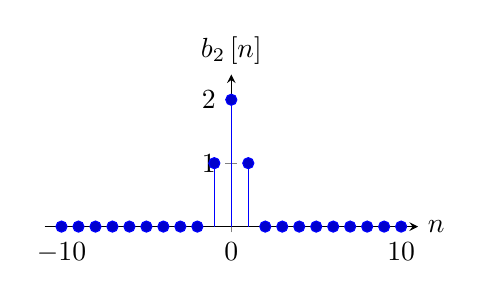
\begin{tikzpicture}
\begin{axis} [width=180pt,height=100pt,
	axis x line=bottom, 
	axis y line=middle, 
	tick align=center,
	every axis x label/.style={at={(current axis.right of origin)},anchor=west},
	every axis y label/.style={at={(current axis.above origin)}, anchor=north east,above=0mm},
	xmin=-11, xmax=11,
	xtick={-10, 0, 10},
	xlabel=$n$,
	ymin=0, ymax=2.4,
	ytick={0,...,2},
	ylabel={$b_2 \left[n\right]$}]
\addplot+[ycomb] plot coordinates {(-10,0) (-9,0) (-8,0) (-7,0) (-6,0) (-5,0) (-4,0) (-3,0) (-2,0) (-1,1) (0,2) (1,1) (2,0) (3,0) (4,0) (5,0) (6,0) (7,0) (8,0) (9,0) (10,0)};
\end{axis} 
\end{tikzpicture}
}
\sublabel{b}{
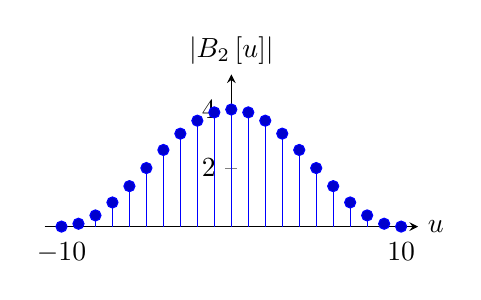
\begin{tikzpicture}
\begin{axis} [width=180pt,height=100pt,
	axis x line=middle, 
	axis y line=middle, 
	tick align=center,
	every axis x label/.style={at={(current axis.right of origin)},anchor=west},
	every axis y label/.style={at={(current axis.above origin)}, anchor=north east,above=0mm},
	xmin=-11, xmax=11,
	xtick={-10, 0,10},
	xlabel=$u$,
	ymin=0, ymax=5.2,
	ytick={0,2,4},
	ylabel={$\left| B_2 \left[ u \right] \right|$},
	color=black]
 \addplot+[ycomb,domain=-10:10,samples=21,samples y=0] 
 ({x}, {abs(2+2*cos(deg(2*pi*x*1/20)))}); 
\end{axis}
\end{tikzpicture}
}
}
\caption{(a) A one-dimensional three-tap approximation to the Gaussian filter ($\left[1,2,1\right]$) and, (b) its Fourier transform for $N=20$ samples. 
%Note that the frequency gain is decreasing monotonically with spatial frequency and it becomes zero at the highest frequency, $G_3 \left[ 10 \right]=0$.
} 
\label{fig:gauss3filter}
\end{figure}


\item All the even binomial filters can be written as successive convolutions with the kernel $\left[1,2,1\right]$. Therefore, their Fourier transform is a power of the Fourier transform of the filter $\left[1,2,1\right]$ and therefore they are also monotonic:
\begin{equation}
B_{2n} \left[u\right] = (2+2 \cos (2 \pi u/N))^n
\end{equation}
The filter transfer function, $B_{2n}$, is real and positive. It is a {\bf zero-phase filter}.
\index{Filter!zero-phase}

\item For all the binomial filters $b_n$, when they are convolved with the wave $\left[1,-1,1,-1,...\right]$, the result is the zero signal $\left[0,0,0,0,...\right]$. This is a very nice property of binomial filters and will become very useful later when talking about downsampling an image (see \chap{\ref{chap:downsampling_and_upsampling}}). 
\end{itemize}

\subsection{2D Binomial Filters}

The Gaussian in 2D can be approximated, using separability, as the convolution of two binomial filters one vertical and another horizontal. For instance:
\begin{equation}
b_{2,2} = b_{2,0} \circ b_{0,2} =  \begin{bmatrix}
  1 ~& 2 ~& 1 \\
\end{bmatrix}\circ \begin{bmatrix}
  1 \\
  2 \\
  1
\end{bmatrix}=
% =
% 
\begin{bmatrix}
  1 ~& 2 ~& 1 \\
  2 ~& 4 ~& 2\\
  1~& 2 ~& 1
\end{bmatrix}
\end{equation}
\marginnote{2D binomial filter:\\[6pt]
%\begin{center}
\centerline{
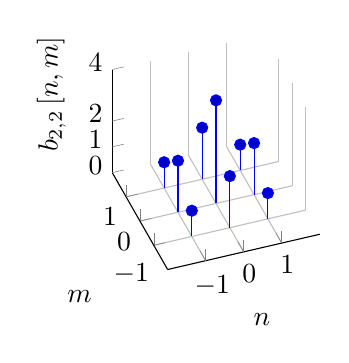
\begin{tikzpicture} 
\begin{axis}[width=120pt,height=130pt,
	mesh/ordering=y varies,
 	%axis x line=middle, 
	%axis y line=middle, 
	%axis z line=middle, 
	%tick align=center,
    xmajorgrids=true,
    ymajorgrids=true,
    zmajorgrids=false,
    zminorgrids=false,
    axis lines*=left, 
	view={-20}{45},
	xmin=-2, xmax=2,
	xtick={-1, 0, 1},
	ymin=-2, ymax=2,
	ytick={ -1, 0, 1}, 
	zmin=0, zmax=4,
	ztick={0, 1,2,4}, 
    xlabel={$n$}, 
    ylabel={$m$}, 
    zlabel={$b_{2,2} \left[n, m \right]$}
	]  
\addplot3+[ycomb]
coordinates { 
(-1,-1,1) (-1,0,2) (-1,1,1)  (0,-1,2) (0,0,4) (0,1,2)  (1,-1,1) (1,0,2) (1,1,1)
};
\end{axis} 
\end{tikzpicture}
}
%\end{center}
%\caption{A discrete 2D signal.} 
%\label{fig:disc2Dsignal_plot}
%\end{figure}
}[-1in]

The filter $b_{2,2}$ has a DC gain of 16, so we will divide the convolution output by 16 so that the output image has a similar contrast to the input image. 

\Fig{\ref{fig:boat_b_noise}} shows an image corrupted by high-frequency checkerboard-pattern noise. The next two images are the result of filtering the noisy image with a $3\times3$ box filter (middle) and with the $b_{2,2}$ binomial filter.
\index{Checkerboard-pattern noise}
The $3\times3$ box filter cannot completely eliminate the noise, while the binomial filter can perfectly cancel this checkerboard noise. Both the box and the binomial filter reduce the resolution of the input image.

\begin{figure}[h]
\centerline{
\includegraphics[width=.32\linewidth]{figures/blur_filters/boat_b_noise.jpg}
\includegraphics[width=.32\linewidth]{figures/blur_filters/boat_c_box.jpg}
\includegraphics[width=.32\linewidth]{figures/blur_filters/boat_d_binomial.jpg}
}
\caption{Image corrupted by a checkerboard-pattern noise (right) and its output to two different blur kernels: (middle) $3\times3$ box filter. (right) Binomial filter $b_{2,2}$.}
\label{fig:boat_b_noise}
\end{figure}


%What is the inverse? can we remove gaussian filter? Show the matrix for some simple case and show it does not behave nicely. 

\section{Concluding Remarks}
%\reviewcomment{To be written.}


The Gaussian and the binomial filters are widely used in computer vision. In particular, the binomial filter $[1,2,1]/4$ (here normalized so that its DC gain is 1), and its 2D extension, are very useful kernels that you can use in many situations like, when you need to remove high-frequency noise, or downsample an image by a factor of 2.
Blur kernels are useful when building image pyramids, or in neural networks when performing different pooling operations or when resizing feature maps. 

\marginnote{Keep the 2D binomial filter close to you:
\begin{equation*}
\begin{bmatrix}
  1 ~& 2 ~& 1 \\
  2 ~& 4 ~& 2\\
  1~& 2 ~& 1
\end{bmatrix}/16
\end{equation*}
}